%--------------------------------------------------
% INSTRUCTIONS / INSTRUÇÕES / INSTRUCCIONES
%--------------------------------------------------

% This file is the official RBIE template for papers written in ENGLISH.

% Para português: use main-pt.tex
% Para español: use main-es.tex

% Do not change the language option in \documentclass.

%----- COMPILATION ENGINE
% Recommended: XeLaTeX or LuaLaTeX
% Do NOT add \usepackage[utf8]{inputenc}: UTF-8 is already native in modern LaTeX and the package is obsolete in this template.

%----- WHAT TO EDIT IN THIS PREAMBLE
% 1. \title -- the title of the paper (English papers show only the English title)
% 2. \author{} -- names, ORCIDs and e-mails

%----- REFERENCES
% 1. The APA 7th edition bibliographic standard is already defined in the 'apalike-sol.bst' style; DO NOT CHANGE IT.
% 2. Add the bibliographic entries to the refs.bib file

%-----  PACKAGES ALREADY LOADED BY THE CLASS (do not redeclare):
    % algorithm, algpseudocode
    % amsmath, amssymb
    % babel
    % caption
    % cuted
    % enumitem
    % etoolbox
    % fontawesome
    % geometry
    % graphicx
    % hyperref
    % listings
    % microtype
    % minted
    % natbib
    % tcolorbox
    % titlesec
    % xcolor
%--------------------------------------------------



% ---- ACCESSIBILITY: tagged PDF / PDF/UA generation ----
% This line MUST remain before \documentclass. It enables the automatic structural tagging required by the Web Content Accessibility Guidelines (WCAG) and by the accessibility guidelines of the Commission for Inclusion, Diversity, and Equity (CIDE) of the Brazilian Computing Society (SBC): headings, lists, tables, and reading order exposed to screen readers. It also sets the PDF language (/Lang) and the PDF/UA-2 standard (ISO 14289-2), the international standard for universal accessibility of PDF files.
% It requires TeX Live 2024 or later (current Overleaf is fine). On TeX Live 2023 or earlier the 'tagging'/'pdfstandard' keys do not exist and compilation fails: in that case, update the distribution. Validate the final PDF (see the Figures section).
\DocumentMetadata{
  lang          = en,
  pdfversion    = 2.0,
  pdfstandard   = ua-2,
  tagging       = off
}

\documentclass[english]{rbie2026}%

% Controls the behavior and position of footnotes
\usepackage[bottom]{footmisc}

%% The tabularray package is the most modern and comprehensive one available for building tables. It replaces the packages tabularx, multirow, multicol, colortbl, and longtable
% https://ctan.org/pkg/tabularray
\usepackage{tabularray}

% Enables the classic 'booktabs' commands: \toprule, \midrule, \bottomrule and \cmidrule inside the tblr environment:
\UseTblrLibrary{booktabs}

% Formats numbers and units according to the International System of Units (SI)
\usepackage{siunitx}

%% Highlight code and demos with l3regex and LPeg
% Enables the \fakeverb{} command, more robust than the native \verb|| command
\usepackage{codehigh}

% Formats web addresses in a monospaced font
\usepackage{url}

% Prevent widow/orphan lines
\clubpenalty  = 100000000
\widowpenalty = 100000000


%----- HEADER INFORMATION. DO NOT EDIT -----------
%----- RESERVED FOR EDITORS ONLY
\jid{RBIE}
\jtitle{Revista Brasileira de Informática na Educação, 20XX, VV:1}
\issn{1414-5685 (print), 2317-6121 (online)}
\doi{10.5753/rbie.yyyy.id}
\copyrightstatement{This work is licensed under a Creative Commons Attribution 4.0 International License}
\jyear{20XX}

\category{Artigo de Pesquisa / Research Paper / Artículo de investigación}

    % --- Alternatives:
    % \category{Artigo estendido / Extended Paper / Artículo extendido}

    % \category{Edição Especial / Special Issue / Edición especial}

% initial page number
% \setcounter{page}{889}
%--------------------------------------------------


%----- ACCESSIBILITY: PDF metadata (recommended) -----
% Fill in the title and authors in PLAIN TEXT (no LaTeX commands, no colors, no "--"). The screen reader announces \pdftitle instead of the file name (already enabled via pdfdisplaydoctitle=true in the class).
\hypersetup{pdftitle={Presenting the RBIE template for 2026: Version for Papers Written in English},
            pdfauthor={Alexandre Direne; José Valente; Liane Tarouco}
            }

%----- PAPER TITLE -------------------------------

% Title in English [Short title]{Long title}
% English papers show only the English title.
\title[Short title of the paper in English]{Presenting the RBIE Template for 2026 -- Version for Papers Written in English}
%--------------------------------------------------


%----- AUTHOR INFORMATION ------------------------
%----- THE ORCID IS MANDATORY FOR EACH AUTHOR IN RBIE

%----- ANONYMOUS SUBMISSION
% For blind review:
% 1. Comment out the whole \author{} block
% 2. In the body of the paper, replace names and affiliations with neutral text
% 3. See Section 3.3.1 for details

\author[
    % Short author/year
    % Choose only ONE of the following three options:
    Direne 20XX (1 author) | Direne \& Tarouco 20XX (2 authors) | Direne et al. 20XX (3 or more authors)]{
    
    % Author 1 info
        \affil{\textbf{Alexandre Ibrahim Direne} \thinspace \orcidlink{0000-0000-0000-0000} \thinspace \textcolor{blue}{\faEnvelopeO} \enspace [{Universidade Federal do Paraná} \thinspace | \thinspace \href{mailto:alexd@inf.ufpr.br}{{\textit{alexd@inf.ufpr.br}}}]}
    
    % Author 2 info
        \affil{\textbf{José Armando Valente} \thinspace \orcidlink{0000-0002-1347-186X} \enspace [{Universidade Estadual de Campinas} \thinspace | \thinspace \href{mailto:jvalente@unicamp.br}{{\textit{jvalente@unicamp.br}}}]}
    
    % Author 3 info
        \affil{\textbf{Liane Margarida Rockenbach Tarouco} \thinspace \orcidlink{0000-0002-5669-588X} \enspace [{Universidade Federal do Rio Grande do Sul} \thinspace | \thinspace \href{mailto:liane@penta.ufrgs.br}{{\textit{liane@penta.ufrgs.br}}}]}
}
%--------------------------------------------------



\begin{document}

%----- Pre-textual elements (front matter)

\begin{frontmatter}
    \maketitle

    % Corresponding mail address
    \begin{mail}
        Departamento de Informática, Centro Politécnico, Universidade Federal do Paraná, R. Evaristo F. Ferreira da Costa, 383--391, Jardim das Américas, Curitiba, PR, 81530-090, Brasil.
    \end{mail}

%----- Abstract and keywords
    % Abstract in English
    % English papers provide only the abstract and keywords in English.
    \begin{abstract-en}
        \textit{Introduction.} Editorial processes in scientific journals require continuous improvement to keep pace with the evolution of research practices and the growing demands for transparency and reproducibility. \textit{Methods.} This article presents the new article template of the Brazilian Journal of Computers in Education -- \emph{Revista Brasileira de Informática na Educação} (RBIE), describing its structure and its methodological recommendations for the most diverse types of research in Computers in Education. The template was developed only in the \LaTeX\ format, covering three languages. \textit{Results.} The template consolidates into a single document conventions that were previously scattered across earlier examples, reducing formatting inconsistencies and simplifying peer review. \textit{Discussion.} The adoption of this template contributes to RBIE's editorial standardization and to the improvement of the methodological quality of submitted articles. For papers written primarily in English, only the abstract in English is required. The abstract should contain between 150 and 300 words.
    \end{abstract-en}

    % Keywords in English
    \begin{keywords}
        Brazilian Journal of Computers in Education; Article template; Scientific writing. [Provide 3 to 10 keywords that facilitate the indexing and retrieval of the article in the main scientific publication databases. Please use semicolons as separators. Keywords must begin with capital letters.]
    \end{keywords}

% EDITION DATES. DO NOT EDIT. RESERVED FOR EDITORS ONLY
    \begin{dates}
        {\sffamily\textbf{Received:}} DD Month YYYY \enspace\textbullet\enspace
        {\sffamily\textbf{Accepted:}} DD Month YYYY \enspace\textbullet\enspace
        {\sffamily\textbf{Published:}} DD Month YYYY
    \end{dates}

\end{frontmatter}

%----- End of pre-textual elements



%------ Start of the manuscript text
\section{Introduction to the RBIE Paper Template}
\label{sec:intro}

We ask authors interested in submitting their research to the Brazilian Journal of Computers in Education (RBIE) to follow the guidelines of this template in order to ensure a standardized presentation. Please read this guide carefully, as it presents important information about ethics, methodological guidance, and formatting instructions. Manuscripts that are not in the appropriate format may be rejected by the editors at any point in the review and publication process.

The author names listed in this template are a posthumous tribute to three researchers who dedicated their careers to the development of Computers in Education in Brazil; none of them took part in its preparation.

\subsection{Scope of RBIE}

RBIE aims to disseminate tools, methods, and practices that support the effective use of technology in the educational process. Although RBIE originally focused exclusively on Computers in Education, it now also welcomes research work on Computing Education.

Despite sharing some common characteristics, it is important to establish the differences between the areas of Computers in Education and Computing Education. As pointed out by \cite{Bispo2020}, research in Computers in Education concerns the use of technological artifacts as mediators in teaching and learning processes, as well as their impacts. Computing Education, in turn, has as its main goal the improvement of the teaching and learning of Computing as a discipline \citep{holmboe2001research}.


\subsection{Recommendations for Writing the Introduction Section}

The ``Introduction'' section, or an equivalent title, should contextualize the research problem, identify the gap the work intends to fill, and explicitly state the contributions of the article. We recommend the following typical organization \citep{ecarnort_writing_article_2015}:

\begin{enumerate}
  \item \textbf{Background (the known).} Present the scenario in which the problem is situated, drawing on evidence from the literature. Avoid generic statements without bibliographic support.

  \item \textbf{Problem and gap (the unknown).} Delimit the specific problem investigated and point out what the literature has not yet fully answered. The gap must be demonstrated, not merely declared.

  \item \textbf{Objective and research questions.} State the general objective of the work. When applicable, present the research questions (RQs) explicitly and in numbered form. This is a well-established practice in Computers in Education and facilitates the reviewers' assessment.

  \item \textbf{Contributions.} List the main contributions of the work concisely. The use of bullet points (\texttt{\textbackslash begin\{itemize\}} or \texttt{\textbackslash begin\{enumerate\}}) is acceptable at this point, at the authors' discretion.

  \item \textbf{Organization of the article.} Optionally, describe in a final paragraph how the remaining sections of the manuscript are structured.
\end{enumerate}

For review or systematic mapping articles, the introduction should additionally include the rationale for conducting a secondary review on the topic, demonstrating that no recent equivalent review exists or that the existing review has relevant limitations.

These structural recommendations are not rigid and may be adapted to the specific characteristics of each research work.


%------------------------------------------
\section{Specific Instructions for \LaTeX}
\label{sec:latex}

The \texttt{rbie2026} class is designed to work with the \texttt{XeLaTeX} and \texttt{LuaLaTeX} engines. Accordingly, the document should be compiled:

\begin{enumerate}
    \item On Overleaf. Go to \textbf{Menu $>$ Settings $>$ Compiler} and set the ``Compiler'' option to \texttt{XeLaTeX} or \texttt{LuaLaTeX}.\footnote{The base engines are called \texttt{XeTeX} and \texttt{LuaTeX}. The combination of these engines with the \LaTeX\ macros forms \texttt{XeLaTeX} and \texttt{LuaLaTeX}.}

    \item On your local installation. Configure your editor or IDE (for example, TeXstudio, TeXworks, or VS~Code) to use \texttt{XeLaTeX} or \texttt{LuaLaTeX} as the compiler. Alternatively, compile from the terminal with \texttt{xelatex file} or \texttt{lualatex file}. There is no need to provide the \texttt{.tex} extension.
\end{enumerate}

The \texttt{rbie2026} class does not work fully with the \texttt{pdfLaTeX} engine. If you try to use it to compile, you will receive warning messages about undefined font packages, and the PDF will be generated with missing glyphs in the icons of the \texttt{fontawesome} package, which relies on Unicode fonts that are not supported by the \texttt{pdfLaTeX} engine.


\subsection{Differences Between \texttt{fontenc} and \texttt{fontspec}}

The \texttt{fontenc} and \texttt{fontspec} packages control font and character handling in \LaTeX. They belong to different eras and compilation engines: \texttt{fontenc} is used with the classic engine (\texttt{pdfLaTeX}), whereas \texttt{fontspec} is mandatory for modern Unicode-based engines (\texttt{XeLaTeX} or \texttt{LuaLaTeX}).

The \textbf{TeX Live} distribution, used by Overleaf to prepare \LaTeX\ documents, installs a wide range of fonts: for example, \textit{TeX Gyre Termes}\footnote{\url{http://www.gust.org.pl/projects/e-foundry/tex-gyre}} is the free and open equivalent of the \textit{Times New Roman} font. For the \texttt{XeLaTeX} or \texttt{LuaLaTeX} engines, it is not mandatory to include the \texttt{fontspec} package. Omitting it makes the engine assume default values for the font and its properties\footnote{For simplicity, the term \textsc{font} is being used as a synonym for the term \textsc{typeface}. However, typography professionals distinguish between the two terms.}.


%------------------------------------------
\section{Manuscript Organization}
\label{sec:organization}

The manuscript must contain \textbf{between 10 and 20 pages}, excluding the complementary declarations, the references, and the appendices.


\subsection{Page Setup}

The paper size must be A4 (210 x 297 mm). The document margins must have the following measurements:

\begin{itemize}
    \item Top: 1{.}0 cm
    \item Bottom: 2{.}0 cm
    \item Left: 1{.}8 cm
    \item Right: 1{.}7 cm
\end{itemize}

These values are already configured in this template. Do not change the margin dimensions, as any text outside the standard may delay or even prevent the publication of your article in RBIE.


\subsection{Titles}


\begin{table*}[ht]
    \centering
    \caption{Examples of title formatting.}
    \label{tab:titulo}
    \begin{tblr}{%
        colspec = {ll},
        cells   = {font=\small}
        }
        \toprule
        \textbf{Incorrect} & \textbf{Correct} \\
        \midrule
        LEARNING PROGRAMMING WITH ONLINE JUDGES
            & Learning Programming with Online Judges \\
        learning programming with online judges
            & Learning Programming with Online Judges \\
        Learning Programming With Online Judges
            & Learning Programming with Online Judges \\
        \bottomrule
        \end{tblr}
\end{table*}


The recommendations below on preparing titles are divided into two types: how to choose the most suitable words and how to format their spelling.

\subsubsection{Choose an Attractive Title}

Craft a strategic title, describing the scope, the design, and the objective of the study. We recommend the following tips \citep{herbst2024structuring,ecarnort_writing_article_2015}:

\begin{enumerate}
  \item \textbf{Be concise and clear.} The title should be short and direct, allowing the reader to quickly infer the content of the publication.

  \item \textbf{Avoid vague wording.} Avoid terms that add no informational value, such as ``a report on\ldots'' or ``a study about\ldots''. If the effects are important, the title should state exactly what they are.

  \item \textbf{Identify the study design.} Specific types of design, such as systematic reviews, systematic mappings, and controlled experiments, should be explicitly identified in the title.

  \item \textbf{Highlight the main finding.} Whenever possible, the title should indicate whether the intervention increases, reduces, or prevents something.

  \item \textbf{Put the most important aspect first.} If the focus is the intervention or the tool being investigated, begin the title with that element to distinguish the article from others on the same topic.

  \item \textbf{Use keywords.} The title should contain the main terms so that the article can be easily retrieved in databases such as SBC-OpenLib (SOL), ACM Digital Library, IEEE Xplore, and Scopus.

  \item \textbf{Spark interest.} The title should be engaging enough to encourage the potential reader to access the full work.

  \item \textbf{Differentiate your work.} The title should make clear how the article contributes to the literature or fills a gap in the knowledge of the field.

  \item \textbf{Identify systematic reviews and mappings.} In the case of secondary and tertiary studies, the title should identify whether the article addresses a systematic mapping (or a systematic review), a tertiary study, an update of an existing systematic review, or whether it includes a meta-analysis \cite{Kitchenham2023_SEGRESS_supp}.
\end{enumerate}


\subsubsection{Format the Title} \label{sec:formatacao_titulo}

The manuscript title must follow these formatting conventions:

\begin{enumerate}
  \item \textbf{Typographic formatting.} For the title in the original language, use the \textit{Roboto} font, size 18pt, left-aligned, with 20pt line spacing and bold style. If the original language of the manuscript is Portuguese or Spanish, the titles in the secondary languages must use the \textit{Roboto} font, size 14pt, left-aligned, 12pt line spacing, bold and italic, in gray (RGB 128, 128, 128).

  \item \textbf{Capitalization (\textit{title case}).} The title should be written with only the initial letter of each word capitalized. The following must have an \textbf{uppercase} initial: the first word of the title (always); nouns, adjectives, verbs, and adverbs; and proper names, including the names of systems, tools, and platforms (e.g., Python, Moodle). The following must remain in \textbf{lowercase} (except when they begin the title): articles (a, an, the); short prepositions (of, in, on, for, by, with, under, over); and conjunctions (and, or, but, that, if).

  \item \textbf{All caps is not allowed.} The title must not be typed entirely in uppercase letters, even to emphasize the work. Table~\ref{tab:titulo} presents examples of incorrect and correct title formatting.

  \item \textbf{Avoid acronyms.} The title should ideally be free of acronyms to ensure clarity and accessibility for the non-specialist reader.

  \item \textbf{Do not end with a period.} Titles are not part of the running text, so they should not end with a period.
\end{enumerate}



\subsection{Author Information}

For the author information (name, ORCID, affiliation, e-mail), use the \textit{Roboto} font, size 10pt, left-aligned, with 8pt line spacing and normal style, without additional spacing.

During the manuscript submission phase, all information that could identify authorship must be suppressed. If the work is accepted, this information must be filled in both the metadata of the submission form and the final version of the manuscript text.


\subsubsection{Manuscript Anonymization}

To ensure the integrity of the double-anonymized review, observe these recommendations for the first version to be submitted:

\begin{itemize}
    \item \textbf{Authors and affiliations.} Omit the names, institutional affiliations, and addresses of all authors. The corresponding fields in the template should be filled in with \textit{Omitted for review}.

    \item \textbf{Acknowledgements.} Suppress the acknowledgements section, as it often identifies funders, advisors, or projects linked to the authors.

    \item \textbf{Funding and grants.} Do not mention funding agencies, process numbers, or research projects that could identify the authors or their institutions.

    \item \textbf{Location of the experiments.} Do not mention the city where the experiments or data collection took place. Mention the state or region only if that information is relevant to the assessment of merit.

    \item \textbf{Institutional platforms and systems.} Do not mention the names of platforms, systems, virtual learning environments, or tools developed by the authors themselves that could identify them. When necessary, use generic designations, such as \textit{the game used} or \textit{the submission platform adopted}.

    \item \textbf{Links and URLs.} Do not include hyperlinks that contain identifying information, such as usernames, names of personal or institutional repositories, or institutional domains. Data or supplementary-material repositories must be anonymized through services such as \textit{Anonymous GitHub} (\url{https://anonymous.4open.science/}) before submission.

    \item \textbf{Self-citations.} When citing your own work, use neutral wording such as \textit{[omitted for review]} in place of the bibliographic reference, avoiding phrases such as \textit{``as we demonstrated in [X]''} or \textit{``in previous work, we investigated...''}.

    \item \textbf{File metadata.} Check and remove the metadata of the PDF file before submission, as it may contain the author's name, the institution, or the software used for editing. On Linux, the command \texttt{exiftool -{}-all= file.pdf} performs this cleanup; on Windows and macOS, the same result can be obtained through the document properties.

    \item \textbf{Figures and screenshots.} Make sure that images, diagrams, and screenshots do not display institutional logos, usernames, e-mail addresses, or any other identifying elements.

    \item \textbf{Questionnaires and research instruments.} If the manuscript describes instruments and questionnaires applied at a specific institution, remove (or generalize) references to the institutional context in the wording and examples reproduced in the text.
\end{itemize}


\subsubsection{Restoration of Authorship after Manuscript Acceptance}

After definitive acceptance of the manuscript, submit the final version with all information restored, including names, affiliations, acknowledgements, and complete references. For each author, the information must be presented in the following sequence:

\begin{enumerate}
    \item Full name of the person, without abbreviations

    \item Link to the ORCID profile (\textit{Open Researcher and Contributor ID})\footnote{\url{https://orcid.org/}}.

    \item When applicable, indicate the corresponding author by means of the symbol \textcolor{blue}{\faEnvelopeO}.

    \item Name of the institution to which the author is affiliated.

    \item E-mail address.
\end{enumerate}


\subsection{Abstract and Keywords}

The abstract is the most-read section of a scientific article. It will probably be the only one read before deciding whether to read the full work. It should offer an overview of the manuscript, covering its objectives, methodology, main results, and conclusions. Here are some recommendations for planning the structure of the abstract, refining its language and style, removing common mistakes, and formatting it.


\subsubsection{Planning the Abstract Structure}

Plan and structure the content of the abstract before developing the sentences, following the guidance below \citep{ecarnort_writing_article_2015}:

\begin{enumerate}
  \item \textbf{Write it last.} Write the abstract after completing all the other sections of the manuscript, since only then is it possible to summarize it accurately.

  \item \textbf{Make it self-contained.} The abstract should work as a standalone document: the reader should understand it fully without needing to consult the full text.

  \item \textbf{Adopt the IMRAD format.} We recommend adopting the standard structure composed of Introduction, Methods, Results, and Discussion (IMRAD) \citep{abstract_Nundy2022}.

  \item \textbf{Answer four fundamental questions:}
  \begin{enumerate}
    \item Why did you start? (Introduction/Objective)
    \item What did you do? (Methods)
    \item What did you find? (Results)
    \item What does it mean? (Conclusions/Implications)
  \end{enumerate}

  \item \textbf{Include real data.} In the results, avoid subjective terms (many, few) and present specific quantitative data, such as \textit{p} values, confidence intervals, percentages, or absolute numbers.

  \item \textbf{Be honest with the results.} Report the main outcomes even if they are not statistically significant; avoid discussing only ``trends'' without empirical support.
\end{enumerate}


\subsubsection{Language and Style}

After outlining the structure of the abstract, revise the linguistic and stylistic choices according to the suggestions below, to make the abstract clearer and more accessible to the reader:

\begin{enumerate}
  \item \textbf{Use the active voice.} Prefer constructions in the active voice (e.g., ``We conducted an experiment\ldots'') rather than the passive voice, as they make reading more direct and objective.

  \item \textbf{Use the appropriate verb tense.} Use the past tense to describe what was done and what was found.

  \item \textbf{Avoid jargon.} Do not use overly complex technical terms or acronyms unfamiliar to the target audience. Define all acronyms at their first occurrence.

  \item \textbf{Prefer simple sentences.} Opt for short, direct declarative sentences, with one main idea per sentence.
\end{enumerate}


\subsubsection{What to Avoid When Writing the Abstract}

The items listed below undermine the quality of an abstract:

\begin{enumerate}
  \item \textbf{Do not include citations.} Abstracts generally should not contain references to other published works. Exceptions: updates of a systematic review, or the continuation or refutation of a specific previous study.

  \item \textbf{Do not cut sentences from the body of the text.} The abstract should be written from scratch, not composed of excerpts copied verbatim from the other sections.

  \item \textbf{Ensure internal consistency.} Check that the data presented in the abstract are identical to those in the tables and in the body of the text.
\end{enumerate}


\subsubsection{Formatting}

To format the abstract and the keywords, follow the guidance below:

\begin{enumerate}
  \item \textbf{Length.} The abstract must contain between \textbf{150 and 300 words}. The last sentence must end with a period.

  \item \textbf{Typography and alignment.} The abstract text must be justified, with single line spacing, without spacing before and after the paragraph, in the \textit{TeX Gyre Termes} font, size 9pt.

  \item \textbf{Keywords.} On the line following the abstract, provide the label ``Keywords:'' in the \textit{Roboto} font, size 9pt, bold. It must be followed by 3 to 10 keywords, in the \textit{TeX Gyre Termes} font, size 9pt, left-aligned, with single line spacing, no spacing before and 24pt spacing after. Use the \textbf{semicolon} as the separator. Keywords must be written with initial capital letters.

  \item \textbf{Required languages.} The number of required abstracts varies according to the main language of the manuscript:

  \begin{itemize}
    \item Papers in \textbf{Portuguese}: in addition to the abstract in Portuguese (native), provide the abstract and keywords also in English (\textit{abstract}) and Spanish (\textit{resumen}), in that order.

    \item Papers in \textbf{Spanish}: in addition to the abstract in Spanish (native), provide only the English version (\textit{abstract}) and the corresponding keywords.

    \item Papers in \textbf{English}: provide only the abstract in English (native). There is no need to provide an abstract or keywords in Portuguese or Spanish.
  \end{itemize}
\end{enumerate}



\subsection{Sections}

The document must be organized in two columns, with the text justified in the \textit{TeX Gyre Termes} font, size 10pt, single line spacing. The first paragraph of a section, subsection, and sub-subsection has no first-line indentation; the remaining paragraphs have a 0{.}71\,cm (20pt) indentation.

Headings follow the capitalization rules of Section~\ref{sec:formatacao_titulo}. The specific formatting of each level is detailed below.


\subsubsection{Section Headings}

A section heading must be written in bold, \textit{Roboto} font, size 14pt, with initial capital letters, left-aligned with single line spacing, with additional spacing of 10pt before and 4pt after. After the heading number, there must be no period.

\subsubsection{Subsection Headings}

A subsection heading must be written in bold, \textit{Roboto} font, size 12pt, with initial capital letters, left-aligned with single line spacing, with additional spacing of 8pt before and 1pt after. After the heading number, there must be no period.

\subsubsection{Sub-subsection Headings}

A sub-subsection heading must be written in bold italic, \textit{Roboto} font, size 11pt, with initial capital letters, left-aligned with single line spacing, with additional spacing of 7pt before and 1pt after. After the heading number, there must be no period.



%------------------------------------------
\section{Related Work}
\label{sec:related-work}

The ``Related Work'' section aims to position the work within the context of the existing literature, ground the methodological choices, and highlight the originality of the contribution. We recommend the following organization:

\begin{enumerate}
  \item \textbf{Literature selection criteria.} Describe, even briefly, how the related works were identified (databases consulted, search terms, period covered). This gives transparency to the literature review process, even in primary research articles, in which the literature review need not follow the rigor of a systematic review, as noted by \cite{Kitchenham2023_SEGRESS}.

  \item \textbf{Thematic organization.} Group the related works by theme or approach, not merely in chronological order. For each group, synthesize what was done, which results were obtained, and which limitations were reported. Avoid writing a sequence of paragraphs in the style \textit{The work of X did Y. The work of Z did W}, without critical or comparative analysis.

  \item \textbf{Differentiation.} Close the section with a paragraph (or subsection) that explicitly articulates how the present work differs from or complements the studies discussed. This paragraph connects the review to the problem stated in the introduction.
\end{enumerate}

For \textbf{systematic review or systematic mapping} articles, we add these recommendations:

\begin{enumerate}
    \item This ``Related Work'' section should be adapted to present the theoretical framework (concepts, models, and theories that ground the review) or a survey of other secondary studies previously conducted. The literature found through the inclusion and exclusion criteria, in turn, should be analyzed in the ``Results'' section (or equivalent).

    \item Check that the database consulted in your review includes RBIE and the SOL library. The absence of these repositories in the search string undermines the coverage of a relevant body of Brazilian scientific output in Computers in Education.
\end{enumerate}



\begin{table*}[ht]
    \centering
    \caption{Citation commands of the \texttt{natbib} package available in the RBIE 2026 template, with examples.}
    \label{tab:natbib}
    \begin{tblr}{%
        colspec  = {Q[l,m]
               Q[l,m,0.4\linewidth]
               Q[l,m]},
        cells    = {font=\small}
        }
        \toprule
        \textbf{Command} & \textbf{Situation} & \textbf{Effect} \\
        \midrule
        %%%
        \textbf{Basic citations} & & \\
        \midrule
        %%%
        % \lstinline$\cite{chave}$ & & \\
          \fakeverb{\cite{key}} &
          Author integrated into the sentence; year in brackets &
          as in \cite{Wohlin2012} \\
        %
          \fakeverb{\citep{key}} &
          Full parenthetical reference at the end of the sentence &
          \citep{Cohen1988} \\
        %
          \fakeverb{\citep[p.~XX]{key}} &
          Parenthetical citation with a specific page or section &
          \citep[p.~15]{Cohen1988} \\
        %%%
        \midrule
        \textbf{Citations with additional notes} & & \\
        \midrule
        %%%
          \fakeverb{\cite[p.~XX]{key}} &
          Author in the sentence; with a specific page or section &
          \cite[p.~15]{Cohen1988} \\
        %
          \fakeverb{\citep[see][]{key}} &
          Parenthetical citation with a textual prefix &
          \citep[see][]{Wohlin2012} \\
        %
          \fakeverb{\citep[see][ch.~Z]{key}} &
          Parenthetical citation with a prefix and a suffix &
          \citep[see][ch.~3]{Wohlin2012} \\
        %
          \fakeverb{\citep[][ch.~Z]{key}} &
          Parenthetical citation with a suffix only &
          \citep[][ch.~3]{Wohlin2012} \\
        \bottomrule
    \end{tblr}
\end{table*}


\subsection{Citations and Bibliographic References}

The reference list must record, accurately and completely, all sources cited in the text, allowing the reader to locate them independently. RBIE adopts the \textbf{APA 7th edition} style \citep{APAStyleTeam2020coronavirus} for formatting references. The guidance below covers the minimum required information, the general style guidelines, and the specific formats by type of work.

\begin{enumerate}
  \item \textbf{Correspondence between citations and reference list.} Every work cited in the body of the article must appear in the reference list, and vice versa. References that are not cited must not be included in the list.

  \item \textbf{Alphabetical ordering.} List the references in alphabetical order by the last name of the first author. In the case of multiple works by the same author (or authorship), order them by year of publication, from oldest to most recent.

  \item \textbf{In-text citation.} Follow the APA~7 author-date format for in-text citations: \textbf{[Last name, Year]} for citations within brackets and \textbf{Last name [Year]} when the author's name is part of the sentence. For works with three or more authors, use the last name of the first author followed by ``\textit{et al.}'' from the first citation onward. For example: Tarouco \textit{et al.} [2015].

  \item \textbf{DOI and URL.} Include the DOI whenever available, formatted as a hyperlink (\texttt{https://doi.org/xxxxx}). In the absence of a DOI, include the stable access URL to the publication. Avoid URLs from search engines, shorteners, or intermediary repositories when the primary source is available.

  \item \textbf{Language of the reference.} References must be recorded in the original language of the work, without translating the titles. When the title is in a non-Latin alphabet, include a transliteration in brackets.

  \item \textbf{Internal consistency.} Adopt a single criterion for abbreviating author names, capitalizing titles, and punctuation, and keep it consistent across all entries in the reference list.

   \item \textbf{Essential information.} Every bibliographic entry must contain these four pieces of information, in this order (APA style):

   \begin{enumerate}
       \item authorship (individuals or institutions)
       \item year of publication
       \item title of the work
       \item place of publication (publisher, journal or venue, URL, institution, etc.)
   \end{enumerate}
\end{enumerate}


\subsubsection{Errors to avoid in references}

\begin{enumerate}
  \item \textbf{Incomplete references.} Do not omit mandatory fields (volume, page numbers, DOI), as this prevents locating the work and undermines the credibility of your work.

  \item \textbf{Citation of secondary sources.} Avoid citing a work through another (``\textit{apud}''). Locate and read the primary source. When this is genuinely impossible, indicate the secondary source in the text and record only the secondary source in the reference list, following the APA~7 guidelines \citep{APAStyleTeam2020coronavirus}.

  \item \textbf{Unstable or restricted-access URLs.} Links to search pages, authenticated sessions, or restricted-access institutional repositories do not allow the source to be retrieved. Prefer DOIs and permanent URLs of open repositories.

  \item \textbf{Preprints presented as published articles.} Preprints have not undergone peer review and should not be referenced as if they were articles published in a journal. If a revised and published version of the same work exists, cite it in place of the preprint.

  \item \textbf{Inconsistency in the spelling of author names.} The same author must not appear with different spellings throughout the reference list (for example, with variation in the number of initials).

  \item \textbf{Omission of the full list of authors.} In the reference list, indicate the names of all authors of each work. Some automated tools erroneously replace the names of the second through last authors with ``\textit{et al.}'' or an equivalent, deviating from the APA~7 style \citep{APAStyleTeam2020coronavirus}. Check and correct this before submitting your manuscript.
\end{enumerate}



\subsection{How to Cite Works in \LaTeX}

RBIE adopts the \texttt{natbib} package for citation management, configured with the \textbf{author-date} style and \textbf{bracket} delimiters. The package provides a set of commands that lets you control precisely how each reference is integrated into the text. Table~\ref{tab:natbib} presents the main available commands, organized by category of use, with examples and the respective typographic effect produced, considering the configuration adopted in this template. It is possible to include additional notes, such as page numbers or sections, through the optional argument of the commands, as illustrated in the table.



%------------------------------------------
\section{Methodology}
\label{sec:methods}

The methodology section should provide enough information for the study to be critically assessed and, when applicable, replicated. The organization varies according to the type of research.

\subsection{Primary Research}

When the manuscript reports primary research (experiment, case study, survey, design research), we recommend addressing the following elements, divided into subsections when necessary:

\begin{enumerate}
  \item \textbf{Research design.} Identify and justify the method adopted, consistent with the research questions. The CEIE/SBC book series\footnote{\url{https://ceie.sbc.org.br/metodologia/}}~\citep{mpcie_vol1_concepcao_pesquisa, mpcie_vol2_pesquisa_quanti, mpcie_vol3_pesquisa_quali} presents the main methods used in the field, among which: controlled experiment and quasi-experiment~\citep{mpcie_vol2_cap2_experimentos}, case study~\citep{mpcie_vol3_cap1_estudo_caso}, survey, \textit{Design Science Research}~\citep{mpcie_vol1_cap5_design_science_research}, action research~\citep{mpcie_vol3_cap2_pesquisa_acao}, and longitudinal study. See \citep{mpcie_vol1_cap4_tipos_pesquisa} for an overview of the research classifications adopted in the field.

  \item \textbf{Participants.} Describe the profile of the participants (number, level of education, institution, point in the program), the recruitment process, and the ethical procedures adopted, including ethics-committee approval, when the experiment involves interventions carried out directly with human beings \citep{mpcie_vol1_cap7_etica}.

  \item \textbf{Instruments and materials.} Describe the instruments used for data collection (questionnaires, computational tools, assessment rubrics), indicating, when applicable, their validity and reliability as previously reported in the literature. According to \cite{Bittencourt_Isotani_2018_Evidencias}, instruments previously validated in the literature are preferable to assessment instruments developed without methodological rigor. For the development and validation of questionnaires in the area of Computers in Education, see \cite{mpcie_vol2_cap6_questionarios}.

  \item \textbf{Procedures.} Describe the sequence of activities carried out, including the schedule, the application conditions, and any experimental control adopted.

  \item \textbf{Data analysis.} Describe the analysis methods employed, indicating the methodological references adopted \citep{creswell2023research}. For \textbf{quantitative approaches}, report the statistical tests and the significance criteria adopted; see \cite{mpcie_vol2_cap9_descritiva} and \cite{mpcie_vol2_cap10_inferencial} for specific guidance. For \textbf{qualitative approaches}, specify the analysis technique adopted, since each one has distinct epistemological assumptions and they are not interchangeable (for example, content analysis~\citep{mpcie_vol3_cap9_analise_conteudo}, discourse analysis~\citep{mpcie_vol3_cap7_analise_discurso}, hermeneutic analysis~\citep{mpcie_vol3_cap8_analise_hermeneutica}, among others). Also report the inter-rater reliability measure, when applicable (for example, Cohen's Kappa~\citep{Cohen1960}).
\end{enumerate}


\subsection{Systematic Review or Systematic Mapping}

The study selection protocol must be described in a structured way, covering the following elements~\citep{Kitchenham2023_SEGRESS_supp, mpcie_vol2_cap3_rsl}:

\begin{enumerate}
  \item \textbf{Research questions (RQs).} Present the RQs that guide the review, preferably structured on the basis of a suitable framework (for example, PICO, PICOC, or equivalent). For guidance specific to the context of Computers in Education, see \citep{mpcie_vol2_cap3_rsl}.

  \item \textbf{Search string and databases.} Present the search string used and the databases consulted, justifying the choices. Report the period covered and the date the search was run.

  \item \textbf{Inclusion and exclusion criteria.} List the criteria explicitly. Ambiguous criteria undermine the reproducibility of the study.

  \item \textbf{Selection process.} Describe the screening stages (reading of title and abstract, full reading) and report the number of studies at each stage. The use of a selection flow diagram is strongly recommended.

  \item \textbf{Data extraction and synthesis.} Describe the data extraction form and the synthesis process adopted. For reviews with two or more researchers, report the inter-rater agreement measure used (for example, Cohen's Kappa~\citep{Cohen1960}).

  \item \textbf{Quality assessment.} When applicable, describe the criteria for assessing the quality of the included primary studies.
\end{enumerate}

Before submitting the manuscript, apply the SEGRESS checklist~\citep{Kitchenham2023_SEGRESS_supp} (\textit{Software Engineering Guidelines for REporting Secondary Studies}) to verify whether all the mandatory elements of the review or mapping are present.

%------------------------------------------
\section{Analysis and Discussion of Results}
\label{sec:analysis}

This section should present the results obtained and the discussion of those results in light of the research questions and the literature. Authors may choose to separate Results and Discussion into distinct sections, provided the organization is consistent with the nature of the study.

\begin{enumerate}
  \item \textbf{Organization by research question.} We recommend structuring the presentation of the results according to the RQs stated in the methodology. Each RQ should be answered with explicit evidence (quantitative data, qualitative excerpts, emerging categories).

  \item \textbf{Presentation of the data.} Use tables and figures to summarize complex data, always referencing them in the text before their presentation. Tables and figures should be self-explanatory through their titles and captions.

  \item \textbf{Analysis of the data contained in the table.} Do not narrate the table in running text, merely repeating the content already presented in tabular form. Interpret the meaning of the values and argue about the implications.

  \item \textbf{Statistical reporting.} For quantitative results, report measures of central tendency and dispersion, the statistical test employed, the \textit{p} value and, mandatorily, the effect size (for example, Cohen's \textit{d}, \(\eta^2\), or equivalent). Statistically significant results, without a report of effect size, are insufficient to assess the practical relevance of the findings.

  \item \textbf{Interpretation and discussion.} Contextualize the results in relation to the reviewed literature. Indicate to what extent the findings corroborate, contradict, or extend previous studies. Avoid letting the discussion be limited to paraphrasing the data already presented.

  \item \textbf{Systematic reviews.} For reviews and mappings, organize the results around the RQs, presenting analytical syntheses (not mere lists of studies). Use visual resources such as charts of distribution by year, theme, method, or publication venue when they contribute to understanding the overall picture of the field.
\end{enumerate}

The subsections below provide methodological and formatting guidelines for non-textual elements in the ``Analysis and Discussion of Results'' section and throughout the manuscript.


\subsection{Non-textual Elements}

Non-textual elements are components of the article that communicate information through visual or structural resources. The most common examples: tables, figures, equations, code listings, and algorithms.

Three rules apply to any non-textual element:

\begin{enumerate}
    \item \textbf{Every element must be discussed in the text.} The non-textual element supports the argument; it does not speak for itself. If the text does not need to discuss it to support a claim, the element is unnecessary and should be removed.

    \item \textbf{The reference precedes the element.} The text must mention the element before it appears on the page.

    \item \textbf{The reference is written with an initial capital letter.} Examples: Table~1, Figure~2, Listing~3, Algorithm~4, Box~5. Equations are the only case in which the number is written in parentheses: Equation~(6).
\end{enumerate}

For all non-textual elements (tables, figures, listings, algorithms, and boxes), the \textbf{caption text} must be formatted as follows: \textit{TeX Gyre Termes} font, size 8pt, justified alignment, with single line spacing, 6pt spacing before the paragraph, and no spacing after. The \textbf{name of the element} and the corresponding numbering follow the same formatting, but must be highlighted in bold. Use a period after the numbering of the element.

\paragraph{Boxed tables.} Some Brazilian editorial conventions, in particular ABNT, distinguish a \textbf{table} (quantitative data, open side borders) from a \textbf{boxed table} (qualitative or mixed data, closed borders). This template treats both as tables, but respects the distinction when authors adopt it consistently in the manuscript.

\paragraph{How to comment on a non-textual element.} Isolated references, such as ``see Table~1'', ``according to Figure~2'', ``as in Listing~3'', are not a scientific discussion. Based on \citet{Moskovitz2023}, we recommend that the passage of running text commenting on each non-textual element carry out the following rhetorical moves. Their combination and order vary according to the section of the article.

\begin{enumerate}
  \item \textbf{Announce.} Tell the reader when to consult the element, referencing it by name and number before it appears on the page. This is the only mandatory move in all sections of the article.

  \item \textbf{Orient.} Briefly describe what the element represents, especially when the type of visualization is not immediately obvious to the target audience. Decide what goes in the running text and what goes in the caption: information that prepares readers \textit{before} they look at the element belongs in the text; information that must be consulted repeatedly \textit{while} they analyze the element belongs in the caption.

  \item \textbf{Observe.} Direct the readers' gaze to the most relevant features, trends, or values. Observations can be specific: in the case of tables and figures, a particular value, peak, \textit{outlier}, or trend; in the case of listings and algorithms, an operation of special interest.

  \item \textbf{Explain.} Interpret the meaning of the observations. Answer the question: why does this pattern occur, and what does it imply for the argument of the article? Observations without an explanation are an incomplete discussion.
\end{enumerate}


\subsection{Tables}

Tables visually organize data that support the argument. A well-constructed table allows the reader to extract information and compare values without needing to resort to the text.

The recommendations below address three topics on table construction: formatting, methodological aspects, and errors to avoid.

\begin{table}[bth]
    \caption{Example of a table caption that spans the width of one column. Table captions should be positioned above. Data source: [indicate].}
    \label{tab:tabela1coluna}
    \centering
    \begin{tblr}{%
        colspec = {cr},
        cells   = {font=\small}
        }
        \toprule
        \textbf{Dimension} & \textbf{Measure (unit)}\\
        \midrule
         1  &  1.6232 \\
         2  &  2.9635 \\
         3  &  3.9724 \\
         4  &  4.9690 \\
         5  &  5.9840 \\
         6  &  6.9842 \\
         7  &  7.9873 \\
         8  &  8.9884 \\
         9  &  9.9873 \\
         10 & 10.9898 \\
         11 & 11.9914 \\
        \bottomrule
    \end{tblr}
\end{table}


\begin{table*}
    \caption{Example of a table caption that spans the width of the two columns of the page. Table captions should be positioned above them. This caption is longer so as to occupy more than one line of space.}
    \label{tab:tabela2colunas}
    \centering
    \vspace{-8pt}
    \begin{longtblr}[%
        label=none,
        note{a} = {\footnotesize{First footnote.}},
        note{$\dag$} = {\footnotesize{This is a second footnote for this table, much longer than the first, to serve as a more complete example for the most varied situations that authors may need.}},
        remark{\footnotesize{Note}} = {\footnotesize{Some general note about the table.}},
        remark{\footnotesize{Source}} = {\footnotesize{Data made up by the creators of the REIC template and reused in the RBIE template.}},
    ]{%
        colspec = {c c c c c c c c c c},
        cells   = {font=\small},
        width = 0.9\linewidth
    }
        \toprule
        \textbf{Number} & \textbf{Vel. (km/h)} &
        $\boldsymbol{\alpha}$ \textbf{(m/s}$\boldsymbol{^2}$\textbf{)} &
        $\boldsymbol{\beta}$ & $\boldsymbol{\gamma}$\TblrNote{a} &
        $\boldsymbol{\delta}$\TblrNote{$\dag$} &
        $\boldsymbol{\epsilon}$ & $\boldsymbol{\zeta}$ &
        $\boldsymbol{\eta}$     & $\boldsymbol{\theta}$ \\*
        \midrule
             1 & 3.5 & 2.0 & 0.20 & $-$0.05 & 0.00 & $-$0.20 & $-$0.05 & 0.20 & 10 \\*
             2 & 2.5 & 1.5 & 0.10 & $-$0.15 & 0.05 & $-$0.15 & ~0.00 & 0.10 & 40 \\*
             3 & 3.0 & 1.8 & 0.20 & $-$0.05 & 0.25 & ~0.05 & ~0.20 & 0.15 & 70 \\*
            \bottomrule
    \end{longtblr}
\end{table*}


\subsubsection{Table Formatting}

\begin{enumerate}
    \item The RBIE template strongly recommends using the \texttt{tabularray}\footnote{\url{https://ctan.org/pkg/tabularray}} package for building tables. It aggregates and improves upon the functionality of several well-known specialized packages: \texttt{tabularx}, \texttt{multirow}, \texttt{multicol}, \texttt{colortbl}, \texttt{longtable}, \texttt{threeparttablex}.

    \item The text size inside the table must be smaller than in the body text (option \fakeverb{cells = {font=\small}}) in the \texttt{tblr} environment.

    \item Tables may occupy one column of the text, like Table~\ref{tab:tabela1coluna}, or span both columns, like Table~\ref{tab:tabela2colunas}.

    \item In tables, captions must be positioned \textbf{above}.

    \item For papers written in English, use the \textbf{period} (\texttt{.}) as the decimal separator.

    \item Tables must not have vertical rules. Horizontal rules should be limited to the header, the footer, and section divisions in larger tables. These recommendations aim to provide a clean look, focused on the data rather than on lines.

    \item The alignment of numeric columns should reflect the nature of the values they contain. Scalar values, which express magnitudes, should be right-aligned (option \texttt{r}), since this alignment lines up the digits by decimal place and facilitates the visual comparison of magnitude. Ordinal values, which merely identify or label the rows, may be aligned according to the authors' style, since they do not represent quantities to be compared with one another. Table~\ref{tab:tabela1coluna} illustrates this distinction: the column of ordinal values, on the left, is centered, whereas the column of scalar values, on the right, is right-aligned.
\end{enumerate}

\subsubsection{Methodological Recommendations}

\begin{enumerate}
  \item \textbf{Informational autonomy.} The caption and footnotes of the table must be sufficient for it to be understood independently of the running text. Abbreviations, units of measurement, and symbols used in the cells must be explained in the notes or in the caption.

  \item \textbf{Numerical precision and consistency.} The values presented must be consistent with those reported in the text and in the other elements of the article. The number of decimal places must be uniform within each column and compatible with the precision of the measuring instrument used. Avoid reporting more decimal places than the precision of the method allows \citep{Cole_too_many_digits}. For samples smaller than 100 individuals, present percentages without decimal places, for example: 9\% (7/79). For samples of 100 or more individuals, one decimal place is adequate, for example: 2.8\% (16/580). In both cases, including the numerator and denominator in parentheses can make your text clearer to the reader.

  \item \textbf{Units of measurement.} Report the unit of measurement of each quantitative column or row, preferably in the header, and not in each individual cell. Use the conventions of the International System of Units (SI) to represent the measures, their symbols, multiples, and submultiples \citep{Inmetro2025SI}. We strongly recommend using the \texttt{siunitx}\footnote{\url{https://ctan.org/pkg/siunitx}} package to format values, units, and derivations according to the SI rules.

  \item \textbf{Completeness of statistical data.} When reporting the results of statistical tests, the table must include, when applicable, the value of the test statistic, the \textit{p} value, and the effect size. Omitting any of these elements undermines the interpretability and reproducibility of the results \citep{Cohen1988}.

  \item \textbf{Identification of missing values.} Blank cells are ambiguous: does the datum not exist, or was it forgotten? Therefore, cells without data must be marked explicitly and consistently, for example with the abbreviation ``N/A'' (not applicable), accompanied by an explanatory note. This methodological recommendation also complies with accessibility guidelines: empty cells hinder table reading by screen readers, and an explicit textual marker makes the absence of data unambiguous for all readers. We do not recommend the use of a dash (---) because screen readers may announce it inconsistently or simply ignore it.
  
  \item \textbf{Meaningful ordering.} Rows and columns must be ordered according to a criterion relevant to the analysis (for example, descending order of frequency, chronological order, or grouping by category).

  \item \textbf{Declaration of data origin and generation tool.} The title, caption, or footnotes of the table must identify the origin of the data presented (own collection, public database, extraction from the literature, etc.) and, when applicable, the tool used to generate or process it (for example, a spreadsheet, a programming language with a specific library, or a database management system). When a generative AI tool is used to produce, complete, or reorganize the data of the table, this must be declared explicitly in the ``Artificial Intelligence (AI) Usage Declaration'', located at the end of the article, as required by the SBC Code of Conduct for authors \citeyearpar{SBC2024conduta_en}. Data generated by AI without independent empirical validation must not be presented as primary research data.
\end{enumerate}


\subsubsection{Errors to Avoid in Tables}

\begin{enumerate}
  \item \textbf{Redundancy with the text.} Do not build tables that merely repeat data already presented in the body of the text. Tables are justified when the data are numerous, multidimensional, or require systematic comparison.

  \item \textbf{Excess of columns or rows.} Excessively wide tables hinder reading and often indicate that the data could be reorganized or split into more than one thematic table.

  \item \textbf{Mixing units without distinction.} Presenting values of different natures (for example, percentages and absolute values) in the same column leads to interpretation errors, unless there is a clear distinction.

  \item \textbf{Vague or overly long titles.} The caption must identify the content of the table precisely. Titles such as ``Results'' or ``Collected data'' are not informative.

  \item \textbf{Absence of a source for secondary data.} When the table presents data extracted from other sources, the reference must be indicated explicitly, either in the title or in a footnote.
\end{enumerate}


\subsection{Figures}

By the term ``figure'', we mean charts, diagrams, flowcharts, screenshots, photographs, and any other visual element that communicates data or processes. The choice and construction of a figure should be guided by the question: \textit{what does this visual element communicate that the text or a table would not communicate with the same efficiency?}

The recommendations below address three aspects of figure construction: formatting, methodological aspects, and errors to avoid. Finally, ethical and legal considerations are presented regarding images that portray research participants, including children.

\subsubsection{Figure Formatting}

\begin{enumerate}
    \item Figures may occupy only one column of the text, like Figure~\ref{fig:figura1coluna}, or span both columns, like Figure~\ref{fig:figura2colunas}.

    \item In figures, captions must be positioned \textbf{below}.

    \item Whenever possible, figures should be submitted in vector format (PDF, SVG, or EPS), and not in \textit{raster} format (PNG, JPEG, TIFF), also known as matrix-based or pixel-based. Vector formats are resolution-independent: the figure remains sharp at any display size, without aliasing. Charts generated by tools such as R, Python (\texttt{matplotlib}, \texttt{seaborn}), SPSS, or Inkscape can be exported directly to PDF or SVG. Photographs and screenshots, by their intrinsic nature, are accepted exceptions in \textit{raster} format, provided they have a minimum resolution of 300 dpi.

    \item \textbf{Alternative text (mandatory).} Every figure must include a textual description through the \texttt{alt} key in the \fakeverb{\includegraphics} command, as shown in Figures~\ref{fig:figura1coluna} and~\ref{fig:figura2colunas}. This text does not appear in the printed PDF, but it is read by screen readers, complying with the Web Content Accessibility Guidelines (WCAG) \citep{W3C2023wcag22}, whose use is recommended by the Commission for Inclusion, Diversity, and Equity (CIDE) of the Brazilian Computing Society (SBC) \citep{sbc2025panorama}. The description must state the figure's purpose, the type of visualization, the axes, and the main trend or finding, and it must transcribe any text embedded in it. Begin the description with the figure's content itself, since screen readers already announce that it is an image. For this reason, avoid saying ``image of'' or ``photo of''.
\end{enumerate}

\begin{figure}
    \centering
    % ACCESSIBILITY: the 'alt' key provides the ALTERNATIVE TEXT read by screen readers (required by Web Content Accessibility Guidelines - WCAG). It does NOT appear in the printed PDF. Describe purpose, chart type, axes, and the main trend/finding. Describe the figure's content directly, without "image of". Avoid subjective interpretation.
    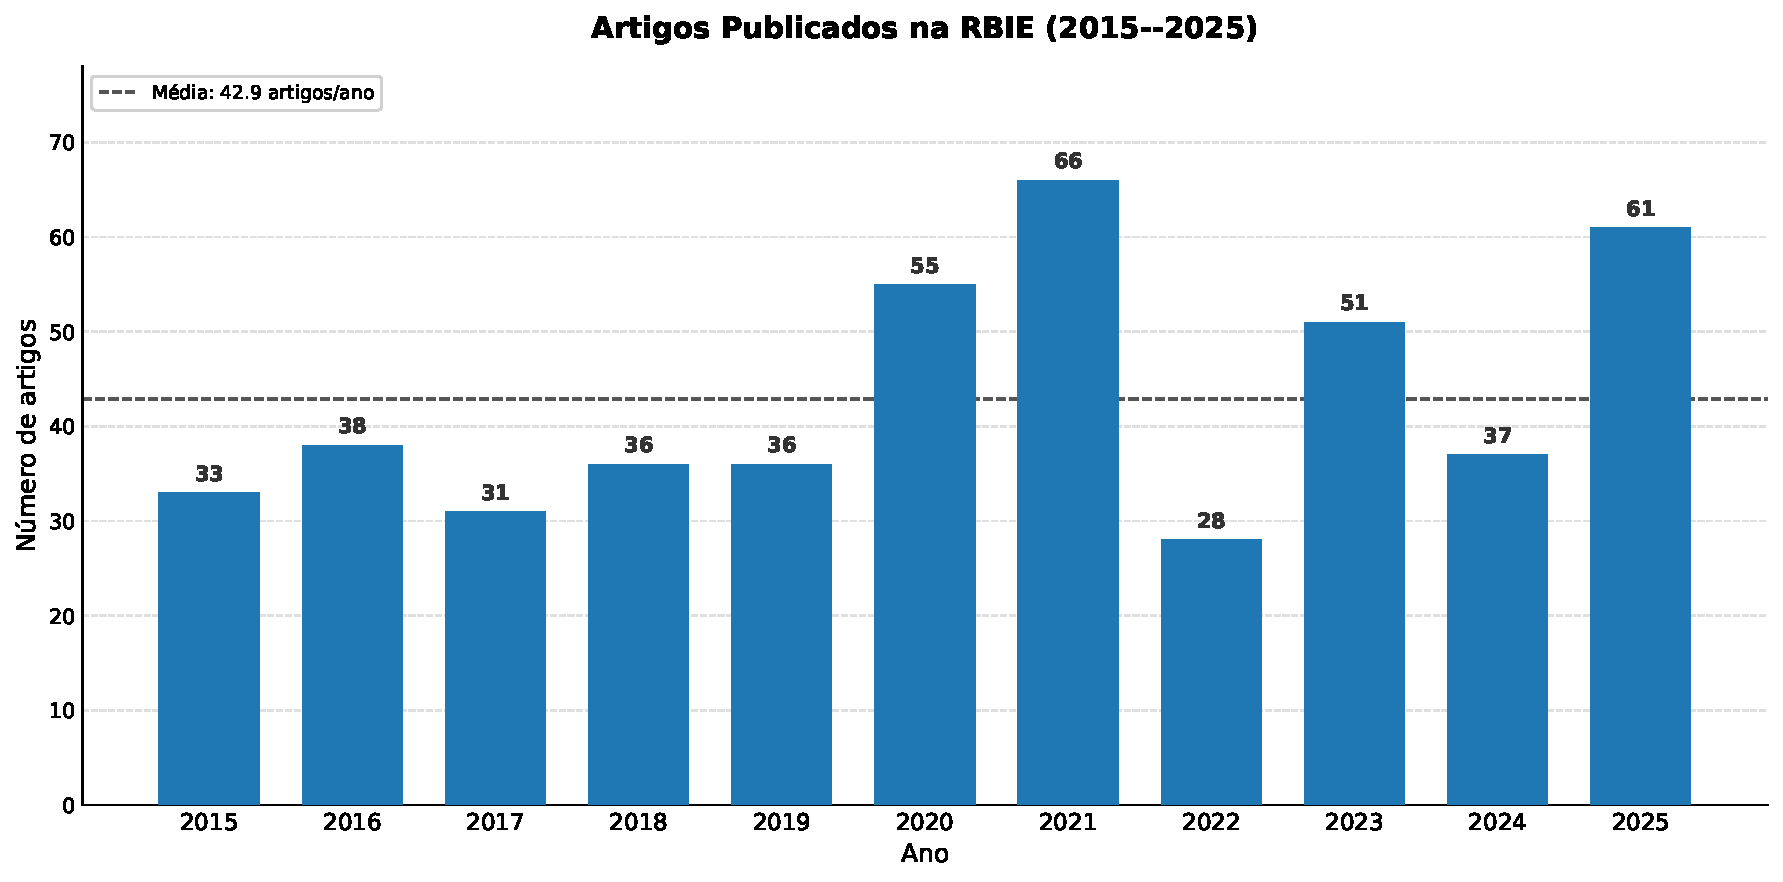
\includegraphics[width=\columnwidth,
      alt={Line chart of the number of articles published in RBIE per year. The horizontal axis shows the years and the vertical axis the number of articles. The series shows an overall upward trend across the period. Replace this description with the one for your figure.}]{img/rbie_artigos_por_ano.pdf}

    % Figure caption, displayed in the printed PDF:
    \caption{Example of a figure caption. Figure captions should be positioned below. Chart generated with the Matplotlib library in Python. Data source: RBIE.}
    \label{fig:figura1coluna}
\end{figure}


\begin{figure*}
    \centering
    % ACCESSIBILITY: see the note on the 'alt' key at the one-column figure above.
    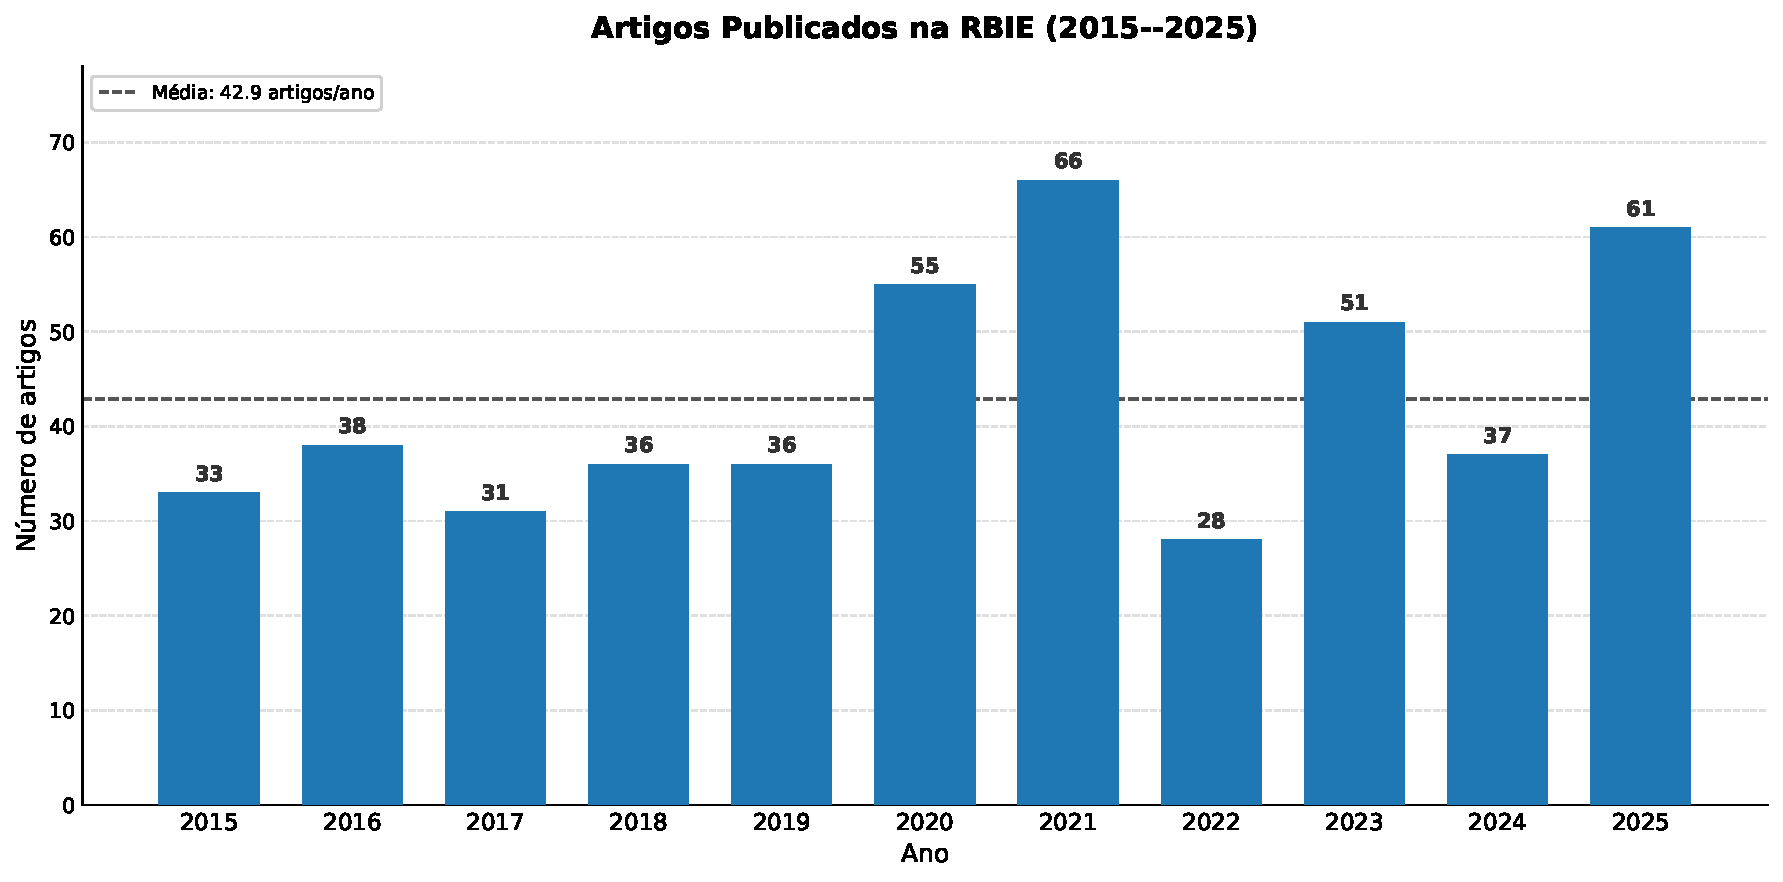
\includegraphics[width=.9\linewidth,
      alt={Line chart of the number of articles published in RBIE per year. The horizontal axis shows the years and the vertical axis the number of articles. The series shows an overall upward trend across the period. Replace this description with the one for your figure.}]{img/rbie_artigos_por_ano.pdf}
    \caption{Example of a figure caption. Figure captions should be positioned below. Chart generated with the Matplotlib library in Python. Data source: RBIE.}
    \label{fig:figura2colunas}
\end{figure*}


\subsubsection{Methodological Recommendations}

\begin{enumerate}
  \item \textbf{Suitability of the figure type to the data.} The type of visualization must be consistent with the nature of the data; otherwise it will distort the interpretation of the data. For example, bar charts are suitable for comparing discrete categories; line charts, for displaying trends along a continuous or temporal variable; scatter plots, for relating two quantitative variables.

  \item \textbf{Informational autonomy.} The caption positioned below the figure must be sufficient for it to be understood independently of the text. Axes, series, symbols, and colors used must be identified in the figure itself or in the caption.

  \item \textbf{Integrity of the visual representation.} The scale of the axes must start at zero when dealing with absolute quantities, unless there is an explicit justification. Truncated or nonlinear scales without an explicit warning distort the perception of the differences between values and constitute a methodological error.

  \item \textbf{Identification of the source for secondary data.} Figures based on data from other sources must indicate the reference explicitly in the caption. Figures reproduced or adapted from other works must indicate the source and, when applicable, the permission of use.

  \item \textbf{Process and flow diagrams.} Flowcharts, sequence diagrams, and concept maps must have consistent notation throughout the article.

   \item \textbf{Data origin and generation tool.} The caption or the text of the manuscript must identify: (A) the source from which the data presented in the figure were extracted; and (B) the software or tool used to generate the figure (for example, a specific R or Python library). When a generative AI tool is used to create, modify, or enhance the figure, this must be declared explicitly in the ``Artificial Intelligence (AI) Usage Declaration'', located at the end of the article, as required by the SBC Code of Conduct for authors \citeyearpar{SBC2024conduta_en}. Figures generated entirely by AI without methodological intervention by the authors (for example, diagrams or infographics produced by a prompt) should be avoided in primary research articles, since they do not constitute a verifiable representation of empirical data. When used for illustrative purposes, they must be identified as such.

  \item \textbf{Figures in systematic reviews.} In systematic review or mapping articles, the study selection flow diagram is a mandatory element. It must record the number of studies at each stage of the screening process, allowing readers to verify the transparency of the study selection process.
\end{enumerate}


\subsubsection{Errors to Avoid in Figures}

\begin{enumerate}
  \item \textbf{Decorative or redundant figures.} Avoid including figures whose content is already fully covered by a table or by the text. Each figure must add information or perspective that the other elements do not offer.

  \item \textbf{Excess of variables in a single figure.} Figures with too many series, colors, or simultaneous dimensions make it hard to draw conclusions. Prefer to split complex visualizations into smaller, more focused figures.

  \item \textbf{Pie charts for four or more categories.} Pie charts make it hard to compare precisely between slices of similar size and color. For four or more categories, bar charts offer greater perceptual precision and should be preferred.

  \item \textbf{Absence of error bars in experimental data.} Charts that present means of experimental data without indicating measures of dispersion (standard deviation, standard error, or confidence interval) hide the variability of the results.

  \item \textbf{Vague captions.} Captions such as ``Results of the experiment'' do not identify the content of the figure. The caption must describe, in a self-contained way, what is being displayed, without readers having to resort directly to the text to extract context.

  \item \textbf{Screenshots as a substitute for data.} Screenshots of tools are acceptable only when the goal is to illustrate the interface itself. Numerical data extracted from tools must be presented in tables or charts built by the authors, not as images of the software output.

  \item \textbf{Three-dimensional effects in charts.} Do not apply 3D effects (perspective, depth, shadow, or extrusion) to bar, pie, line, or scatter charts. They visually distort the proportions between the values, hinder the reading of the magnitudes represented, and add no information to the chart. Three-dimensionality is justified only when the data effectively have three analytical dimensions to represent.
\end{enumerate}


\subsubsection{Recommendations Regarding Photographs of People}

The publication of photographs of research participants is regulated by the following protection and privacy standards:

\begin{itemize}

  \item \textbf{In Brazil:}

  \begin{itemize}
    \item General Personal Data Protection Law (LGPD) \citep{LGPD2018};

    \item Statute of the Child and Adolescent (ECA) \citep{ECA1990};

    \item Law No. 14,874/2024 \citep{brasil2024lei14874}, regulated by Decree No. 12,651/2025 \citep{brasil2025decreto12651}, which governs research with human beings and establishes the National System of Research Ethics with Human Beings, the legal framework in force since 2024;

    \item CNS Resolutions No. 466/2012 \citep{cns2012resolucao466} and No. 510/2016 \citep{cns2016resolucao510}, which remain valid as an ethical reference to the extent that they do not conflict with the new legal framework, during the transition period. Resolution No. 510/2016 deals specifically with research in the Human and Social Sciences, the field into which most Computers in Education studies fall; Resolution No. 466/2012 is the general framework and applies on a subsidiary basis.
  \end{itemize}

  \item \textbf{Internationally:}

  \begin{itemize}
    \item General Data Protection Regulation of the European Union (GDPR) \citep{GDPR2016};

    \item Ethical guidelines of the \textit{American Psychological Association} (APA).
  \end{itemize}

\end{itemize}


A photograph of a research participant is not merely a decorative element in the manuscript. It is sensitive personal data with ethical, legal, and human implications. Before including any image that portrays human beings, mentally answer the following questions:

\begin{enumerate}
  \item Is this image scientifically necessary?

  \item Do I have documented authorization to publish it?

  \item Does the publication preserve the dignity of those who appear in it?
\end{enumerate}

The recommendations below guide this process.

\begin{enumerate}
  \item \textbf{Scientific necessity of the image.} The inclusion of photographs of people must be justified by the scientific contribution of the image to the argument of the article. Example: photographs of participants interacting with learning tools or environments are pertinent when the spatial or behavioral context is relevant to the analysis. Photographs of team gatherings or merely illustrative ones must not be included.

  \item \textbf{Free, informed, and documented consent.} The publication of photographs that allow the identification of adults requires a specific informed consent form (ICF) for image use, distinct from the general research ICF. The signed document must be retained by the researchers and be available for verification by the RBIE editorial team.

  \item \textbf{Authorization of legal guardians for photographs of children.} For images of minors under 18 years of age, consent must be obtained from the parents or legal guardians, in accordance with the ECA (article 17). It is additionally recommended to obtain the assent of the child, when their maturity allows, in accordance with CNS Resolution No. 466/2012 \citep{cns2012resolucao466}.

  \item \textbf{Anonymization when consent is not obtained.} When it is not possible to obtain consent, or when exposing the identity is not necessary to the scientific argument, the photograph must be anonymized before submission. Acceptable techniques include blurring or occluding the face region and other identifying elements (tattoos, uniforms with names, badges). Anonymization must be applied to all identifiable people in the image, not only to the focal participant.

  \item \textbf{Declaration in the article.} Authors must declare, in the ``Declarations'' or ``Methodology'' section, that consents for image use were obtained and that the study was submitted to and approved by the competent Institutional Review Board (IRB). \textbf{This declaration is mandatory for publication of the study in RBIE.} We recommend following the current guidance of the authors' IRB regarding the submission flow and the responsible body.

  \item \textbf{Attention to contexts of vulnerability.} Photographs that portray participants in a situation of vulnerability (students with learning difficulties, Indigenous populations, children at risk) require redoubled care. In these cases, even with consent, authors must assess whether publishing the image preserves the dignity of the participants and does not expose them to additional risks arising from the circulation of the article.
\end{enumerate}


%------------------------------------------
\subsection{Equations}

To insert equations in the text, we recommend that authors observe the following guidance:

\begin{enumerate}
  \item \textbf{Numbering.} Number all equations that are referenced in the text. If only a single equation is used in the text, then the numbering may be omitted. Use the \texttt{equation} environment to control the numbering automatically:

\begin{equation}
  \label{eq:fmeasure}
  F_1 = 2 \cdot \frac{\text{Precision} \times \text{Recall}}
                     {\text{Precision} + \text{Recall}}
\end{equation}

  \item \textbf{Reference in the text.} Every equation must be referenced in the text before its presentation; otherwise, it will be merely a decorative element and therefore disposable. Use the \fakeverb{\eqref{label}} command, which will produce, for example: ``as in Equation~\eqref{eq:fmeasure}''. Note that this command, unlike \fakeverb{\ref}, automatically produces a pair of parentheses around the number of the equation.

  \item \textbf{Definition of variables.} Define all variables and symbols immediately after the equation. For example: ``where $F_1$ is the harmonic mean between precision and recall''. Do not assume that readers know the notation adopted.

  \item \textbf{Inline equations.} For short expressions integrated into the running text, use inline math mode (\fakeverb{$...$}). For example: the accuracy was $\hat{y} = 0.87$. Reserve the \texttt{equation} and \texttt{align} environments for expressions that deserve their own emphasis.

  \item \textbf{Alignment of multiple equations.} When presenting a system of equations or a step-by-step derivation, use the \texttt{align} environment to align the equals signs:

\begin{align}
  \text{Precision} &= \frac{TP}{TP + FP} \\
  \text{Recall} &= \frac{TP}{TP + FN}
\end{align}

  \item \textbf{Punctuation.} Equations are part of the syntactic structure of the text and must receive appropriate punctuation. If the equation ends a sentence, end it with a period. If the sentence continues after the equation, use a comma.

  \item \textbf{Consistent notation.} Keep the same notation for the same variable throughout the entire article. For example, scalar variables should be written in italics ($x$), vectors in bold ($\mathbf{v}$), and matrices in bold uppercase ($\mathbf{A}$), according to the standard mathematical convention \citep{AMS2021handbook, Higham2020handbook, Knuth1989mathematical}.
\end{enumerate}


\subsection{Program Code}

We recommend the following guidance for presenting code or pseudocode listings:

\begin{enumerate}

  \item \textbf{Recommended environment.} We recommend the \texttt{minted}\footnote{\url{https://ctan.org/pkg/minted}} package to display code snippets with syntax highlighting. The package is already loaded by the \texttt{rbie2026} class and does not need to be declared in the preamble. Listing~\ref{lst:exemplominted} illustrates a function in Python.


\begin{listing}[H]
    \caption{Example of code formatted with the \texttt{minted} package.}
    \label{lst:exemplominted}
    \begin{minted}{python}
def soma(a, b):
    return a + b
    \end{minted}
    \vspace{-12pt} % removes unnecessary space between the listing and its caption below
\end{listing}

  \item \textbf{Short inline snippets.} To insert identifiers, reserved words, or short expressions in the middle of the text, choose the command according to the content:

  \begin{itemize}
    \item For simple names, without \LaTeX\ special characters, use \fakeverb{\texttt{...}}. Example: ``the \texttt{compute\_mean()} function returns a value of type \texttt{float}''.

    \item To display snippets that contain special characters (backslash, braces, underscore, hash sign), use \fakeverb{\fakeverb{...}}, which dispenses with manually escaping those characters. Unlike \fakeverb{\verb||}, it also works inside captions, footnotes, and table cells. Example: \fakeverb{\fakeverb{\citep[p.~15]{key}}} produces \fakeverb{\citep[p.~15]{key}}. The command is provided by the \texttt{codehigh} package, already loaded in the preamble; the only requirement is that the braces inside the argument be balanced.
  \end{itemize}

  \item \textbf{Pseudocode.} When the goal is to describe an algorithm in a language-independent way, prefer pseudocode over a snippet of real code. In that case, adopt a consistent notation and declare the conventions used in the caption or in the text. Algorithm~\ref{alg:soma} illustrates a pseudocode.


\begin{algorithm}
    \caption{Sum algorithm}
    \label{alg:soma}
    \begin{algorithmic}[1]
        \State $s \gets a + b$
    \end{algorithmic}
\end{algorithm}


  \item \textbf{Caption and reference.} The caption of code blocks must be positioned \textbf{below}, following the same convention as figures.

  \item \textbf{Length of the snippet.} Include only the code snippet strictly necessary to illustrate the point discussed in the text. Avoid reproducing entire files or long functions. Instead, make the complete code available in a public repository, reported in the ``Declarations'', in the ``Availability of data and materials'' section.

  \item \textbf{Identifiers.} Adopt a standard for the names of variables, functions, and comments throughout the entire article. For papers written in English, identifiers in English are preferable, except when the code reproduces a real artifact already published in another language.
\end{enumerate}


\subsection{Numbered Text Boxes}

Text boxes can be useful for controlling the numbering of, and referencing, a sequence of prompts, search strings, or another artifact in running-text form. Box~\ref{inputbox:prompt} shows an example of how a prompt can be presented in an RBIE article.

To insert a box in \LaTeX, use the custom environment \texttt{inputbox}, built on the \texttt{tcolorbox}\footnote{\url{https://ctan.org/pkg/tcolorbox}} package.

The text of the box must be written in the \textit{TeX Gyre Termes} font, size 9pt, justified alignment, with single line spacing, no spacing before or after the paragraph.


\begin{inputbox}{Example caption of a text box: prompt for the synthetic generation of an activity in a programming course. Source: own elaboration. \label{inputbox:prompt}}
    You are a teacher delivering a course on \textbf{\textcolor{variablecolor}{\{SUBJECT\}}} and you want to build a practical activity for your students. Note that your students do not necessarily have a strong background in mathematics and computer science, so the difficulty level of the task should be \textbf{\textcolor{variablecolor}{\{INTERMEDIATE\}}}. The practical activity should be composed of \textbf{\textcolor{variablecolor}{\{NUM\_TASKS\}}} tasks. Format the output in markdown.
     % \label{}
\end{inputbox}



%------------------------------------------
\section{Research Limitations}
\label{sec:limitations}

The declaration of research limitations is a requirement of scientific integrity and must be presented in a reflective, not defensive, manner. To facilitate communication, we recommend adopting the taxonomy of \cite{Wohlin2012}, as it is widely used in empirical research in Software Engineering and Computers in Education. It comprises the following dimensions:

\begin{enumerate}
  \item \textbf{Internal validity.} Discuss factors that may have influenced the results in an uncontrolled way, such as maturation effects, participant selection bias, contamination between groups, or sample loss.

  \item \textbf{External validity.} Discuss the limits of generalization of the results, considering the profile of the participants, the institution, the cultural context, and the period in which the study was conducted. Do not claim generalizability that the data do not support.

  \item \textbf{Construct validity.} Discuss the extent to which the instruments used actually measure the constructs they are meant to measure. For adapted or translated scales, indicate the validation procedures adopted.

  \item \textbf{Conclusion validity.} Discuss aspects related to the statistical power of the study, the reliability of the measures, and the consistency of the analysis process.
\end{enumerate}

For systematic reviews and mappings, the limitations must additionally address \citep{Kitchenham2023_SEGRESS_supp}: possible publication bias, limitations of the databases consulted, language restrictions applied, and the subjectivity inherent in the data extraction and synthesis process.



%------------------------------------------
\section{Open Science, Reproducibility, and Availability of Materials}
\label{sec:openscience}

RBIE encourages the adoption of open science practices as a way to increase the transparency, reproducibility, and impact of published research. The guidance below applies to the two phases of the editorial process.


\subsection{Submission Phase}

For the purposes of the double-anonymized review, if your work involves artifacts in repositories, then adopt these precautions:

\begin{itemize}
    \item \textbf{Anonymized repositories.} Supplementary materials, datasets, source code, and research instruments must be made available through anonymized repositories, such as \textit{Anonymous GitHub} (\url{https://anonymous.4open.science/}), so as not to compromise the anonymity of the submission.

    \item \textbf{Pre-registrations.} If the study was pre-registered on platforms such as OSF (\url{https://osf.io/}) or AsPredicted (\url{https://aspredicted.org/}), the link must be anonymized or omitted in the submitted version, and restored in the final version.

    \item \textbf{Sensitive data.} Data involving human participants must not be made publicly available without proper ethical treatment. Check that the collection protocol complies with Law No. 14,874/2024 \citep{brasil2024lei14874} and Decree No. 12,651/2025 \citep{brasil2025decreto12651}, with CNS Resolutions No. 466/2012 \citep{cns2012resolucao466} and No. 510/2016 \citep{cns2016resolucao510}, which remain valid to the extent that they do not conflict with the new legal framework, and with the LGPD \citep{LGPD2018}.
\end{itemize}


\subsection{Final Version Delivery Phase}

After the review rounds and the acceptance of the article for publication in RBIE, remove the authorship anonymization in the final version. In addition, make all materials and artifacts necessary for the reproducibility of the research available in the Declarations of the article, in the ``Availability of data and materials'' section, observing the following precautions:

\begin{itemize}
    \item \textbf{Research data.} Make the datasets used in the analyses available in open-access repositories with the assignment of a permanent DOI, such as Zenodo (\url{https://zenodo.org/}), OSF (\url{https://osf.io/}), Dryad (\url{https://datadryad.org/}), Figshare (\url{https://figshare.com/}), or a relevant institutional repository. Indicate in the final version of the manuscript the repository, the DOI, and other relevant information.

    \item \textbf{Source code and scripts.} Share analysis code, processing scripts, and implementations in public repositories (e.g., GitHub, GitLab), preferably with an explicit open license, such as MIT, Apache 2.0, or CC BY 4.0.

    \item \textbf{Research instruments.} Make questionnaires, interview scripts, assessment rubrics, and other instruments used in data collection available as supplementary material, either in the article's online repository or as an appendix to the manuscript.

    \item \textbf{Intervention materials.} Share activities, exercises, problems, and other pedagogical materials described in the study in a way that allows the replication of the research by other groups.

    \item \textbf{Computational reproducibility.} When the research involves computational analyses, use reproducible environments, such as Docker containers, Conda environments, or Jupyter notebooks, accompanied by clear execution instructions.

    \item \textbf{Licensing.} All materials made available must have an explicit license of use. For data and documents, the Creative Commons CC BY 4.0 license is recommended; for software, an open-source license recognized by the OSI (\url{https://opensource.org/}).

    \item \textbf{Availability declaration.} At the end of the manuscript, include the section titled \textit{Availability of data and materials}, indicating where the resources can be accessed, or justifying, when applicable, the impossibility of sharing.

    % \item \textbf{Preprints.} The submission of preprints to servers such as SocArXiv (\url{https://osf.io/preprints/socarxiv}) or EdArXiv (\url{https://osf.io/preprints/edarxiv}) is permitted, provided the preprint does not identify the authors during the anonymous review period.
\end{itemize}

The adoption of these practices contributes to the scientific quality of published works and is aligned with the international open science guidelines:

\begin{itemize}
    \item UNESCO Recommendations on Open Science \citep{UNESCO2022en}; and
    \item FAIR Principles (\textit{Findable, Accessible, Interoperable, Reusable}) of data management \citep{FAIRprinciples2016}.
\end{itemize}



%------------------------------------------
\section{Conclusion and Future Work}
\label{sec:conclusion}

The conclusion should revisit the investigated problem, synthesize the main findings in relation to the research questions, and present the practical and theoretical implications of the work. We recommend the following organization:

\begin{enumerate}
  \item \textbf{Revisiting the problem and the objective.} In one or two initial paragraphs, recapitulate the problem that motivated the study and the proposed objective. Do not reproduce excerpts from the introduction verbatim.

  \item \textbf{Synthesis of the results.} Present the main findings in an integrated way, directly answering the research questions. The conclusion is not the place to introduce new data or analyses not discussed previously.

  \item \textbf{Pedagogical implications.} Discuss the implications of the results for teaching practice, for the design of tools, or for research in the field. Highlight the practical applicability, transferability, and impact of the findings on education. Distinguish, when pertinent, the implications for researchers, teachers, and other education professionals.

  \item \textbf{Future work.} Indicate the research directions opened up by the present work. Future work should follow naturally from the limitations identified and the results obtained, not constituting a wish list disconnected from the study.
\end{enumerate}

Finally, we hope that the information contained in this paper template helps in the preparation of your manuscript. If you find any inconsistency or need further information, please contact the RBIE editorial team.



%------------------------------------------
% Mandatory and optional declarations that complement the text
\begin{declarations}

\begin{acknowledgements}
THIS DECLARATION IS OPTIONAL. The names listed as authors of this template are a posthumous tribute to three researchers who dedicated their careers to the development of Computers in Education in Brazil. Alexandre Ibrahim Direne (1960--2017), José Armando Valente (1948--2025), and Liane Margarida Rockenbach Tarouco (1947--2025) did not participate in the preparation of this template and are not responsible for any part of its content. All responsibility for the material presented here lies with the editors of RBIE.
\end{acknowledgements}

\begin{funding}
THIS DECLARATION IS OPTIONAL. This research was funded by lorem ipsum dolor sit amet, consectetur adipiscing elit.
\end{funding}

\begin{contributions}
THIS DECLARATION IS MANDATORY. Authors must describe their contribution using the CRediT Taxonomy\footnote{\url{https://credit.niso.org/}}, as in this example: AID contributed to the conception of this study. JAV and LMRT conducted the experiments. AID is the main contributor and writer of this manuscript. All authors read and approved the final manuscript.
\end{contributions}

\begin{interests}
THIS DECLARATION IS MANDATORY. If there are no conflicts of interest, the authors must declare: ``The authors declare that they have no conflicts of interest''. Otherwise, the declaration must be: ``The authors declare that they have the following conflicts of interest: lorem ipsum dolor sit amet, consectetur adipiscing elit.''
\end{interests}

\begin{materials}
THIS DECLARATION IS MANDATORY.
  If the authors are making their data and/or code openly available, the declaration must be: ``The datasets (and/or software) generated and/or analyzed during the current study are available at \ldots''. Otherwise, the declaration must be: ``The datasets (and/or software) generated and/or analyzed during the current study will be made available upon request''.
\end{materials}

\begin{aiusagedeclaration}
THIS DECLARATION IS MANDATORY. In compliance with the SBC Code of Conduct for authors \citeyearpar{SBC2024conduta_en}, ``the use of Generative AI tools and technologies to generate content, in the writing and/or revision of the content of articles, must be declared explicitly in the work''. Authors must list the tools and describe where they were used, for example: initial drafting, text revision, idea generation, data analysis, translation, creation of figures/tables, script generation, or other stages. ``These tools cannot be listed as authors of the article. The use of such tools does not exempt the authors from responsibility for all of its content, including in the event that plagiarism is identified''. If no generative AI tool was used at any stage of the development of the work, state this explicitly.
\end{aiusagedeclaration}


\begin{furtherinformation}
THIS DECLARATION IS DESIRABLE. Include relevant additional information, such as, for example, the approval by a Research Ethics Committee. If there is nothing to add, this declaration may be removed.

For award-winning articles, adapt this example declaration: This publication is an extended version of the best paper of the $<$event name$>$ ($<$EVENT ACRONYM$>$ 20XX), titled \textit{``Title of the original paper''}. DOI: \url{https://doi.org/xxxxx.xxxx}.

\end{furtherinformation}
\end{declarations}


%%%% Bibliography style
\bibliographystyle{apalike-sol}

%%%% Bibliographic reference database
\bibliography{refs}


%%%% Appendices
\section*{Appendix A}

Appendices and annexes are complementary materials that expand or support the content of the article without interrupting the flow of reading. The distinction between the two types depends on authorship:

\begin{itemize}
  \item \textbf{Appendix (most common case):} material prepared by the authors themselves, such as questionnaires developed for the research, interview scripts, experimental protocols, assessment rubrics, or detailed descriptions of implementations.

  \item \textbf{Annex:} an external document incorporated into the article by reference, such as normative resolutions, standardized institutional forms, or validated instruments produced by third parties.
\end{itemize}

Every appendix or annex must be referenced in the body of the text. Materials that are not mentioned in the text must be omitted. Appendices and annexes must appear after the bibliographic references, without starting a new page, identified by a sequential uppercase letter: Appendix~A, Appendix~B, Annex~A, Annex~B.

\end{document}
